\documentclass{report}
\usepackage[utf8]{inputenc} %encodage entrée
\usepackage{endnotes} %notes de fin
\usepackage{graphicx} %images
\usepackage[usenames,dvipsnames]{color} %couleurs
\usepackage{listings} %mise en forme de code source
\usepackage{xfrac}
\renewcommand\theequation{\arabic{equation}}
\usepackage{tabularx} % modifier la taille des cellules des tableaux
\usepackage{upquote}
\usepackage{textcomp}
\usepackage{pdfpages}
\usepackage[frenchb]{babel} %langue
\usepackage{amsmath} %affichage des matrices
\usepackage{lipsum} %génération de lipsum
\usepackage{verbatim} %code source
\usepackage{moreverb} %amélioration du package verbatim
\usepackage{titlesec} %formatage des chapitres
\titleformat{\chapter}[hang]{\bf\huge}{\thechapter}{2pc}{}
\usepackage[a4paper]{geometry} %mise en page
% \usepackage{varioref,amssymb,float} % polices 
% \usepackage{pgf,tikz} % permet de créer comme pstricks des figures en code LateX 
% \usetikzlibrary{calc} 
% \usepackage{pgflibraryarrows} % librairie liée à tikz 
% \usepackage{pgflibrarysnakes} 
% \usepackage{xcolor} % module de couleur pour tikz 
\geometry{hscale=0.8,vscale=0.8,centering}
%\lstinputlisting[language=Python, firstline=37, lastline=45]{source_filename.py}
\title{Algorithmes numériques -- Rapport \\ \vspace{0.5cm}Interpolation et Approximation}
\author{Axel Delsol, Pierre-Loup Pissavy}
\date{Décembre 2013}
\lstset{literate=
   {á}{{\'a}}1 {é}{{\'e}}1 {í}{{\'i}}1 {ó}{{\'o}}1 {ú}{{\'u}}1
   {Á}{{\'A}}1 {É}{{\'E}}1 {Í}{{\'I}}1 {Ó}{{\'O}}1 {Ú}{{\'U}}1
   {à}{{\`a}}1 {è}{{\`e}}1 {ì}{{\`i}}1 {ò}{{\`o}}1 {ò}{{\`u}}1
   {À}{{\`A}}1 {È}{{\`E}}1 {Ì}{{\`I}}1 {Ò}{{\`O}}1 {Ò}{{\`U}}1
   {ä}{{\"a}}1 {ë}{{\"e}}1 {ï}{{\"i}}1 {ö}{{\"o}}1 {ü}{{\"u}}1
   {Ä}{{\"A}}1 {Ë}{{\"E}}1 {Ï}{{\"I}}1 {Ö}{{\"O}}1 {Ü}{{\"U}}1
   {â}{{\^a}}1 {ê}{{\^e}}1 {î}{{\^i}}1 {ô}{{\^o}}1 {û}{{\^u}}1
   {Â}{{\^A}}1 {Ê}{{\^E}}1 {Î}{{\^I}}1 {Ô}{{\^O}}1 {Û}{{\^U}}1
   {œ}{{\oe}}1 {Œ}{{\OE}}1 {æ}{{\ae}}1 {Æ}{{\AE}}1 {ß}{{\ss}}1
   {ç}{{\c c}}1 {Ç}{{\c C}}1 {ø}{{\o}}1 {å}{{\r a}}1 {Å}{{\r A}}1
   {€}{{\EUR}}1 {£}{{\pounds}}1
}
\lstdefinestyle{customc}{
   belowcaptionskip=1\baselineskip,
   breaklines=true,
   frame=L,
   xleftmargin=\parindent,
   language=C,
   showstringspaces=false,
   basicstyle=\footnotesize\ttfamily,
   keywordstyle=\bfseries\color{ForestGreen},
   commentstyle=\itshape\color{Plum},
   identifierstyle=\color{NavyBlue},
   stringstyle=\color{Orange},
   numbers=left,
   caption=Code : \lstname,
   captionpos=b,
}
\lstset{
upquote=true,
columns=flexible,
basicstyle=\ttfamily,
}
\addto\captionsfrench{\renewcommand{\figurename}{\textsc{Graphique}}}
\addto\captionsfrench{\renewcommand{\tablename}{\textsc{Tableau}}}
\renewcommand{\thefigure}{\thesection.\arabic{figure}}
\renewcommand{\thetable}{\thesection.\arabic{table}}
\renewcommand{\lstlistingname}{\textsc{Figure}}
\lstdefinestyle{apercu}{
  xleftmargin=2cm,
  xrightmargin=2cm,
  frame=single,
  breaklines=true,
  breakatwhitespace=true,
  breakindent=5pt,
  postbreak=\space,
  captionpos=b,
  escapeinside={\%*}{*)},
  showstringspaces=false,
  caption=Apercu : \lstname,
}
\begin{document}
  \maketitle
  \tableofcontents

  \chapter{Préambule}
    \section{Structure du programme}
    Nous avons conçu un programme principal avec menus, présenté sous la forme suivante :
    \begin{lstlisting}[style=apercu, name=Menu Principal]
Menu principal : Interpolation et Approximation

Entrez n le nombre de points : 2
%*\textit{(Saisie de la série de points...)}*)

%*\textit{(Affichage du tableau correspondant...)}*)
Quelle résolution utiliser ?
1- Newton
2- Neuville
3- Régression Linéaire par une droite
4- Régression Linéaire par une fonction exponentielle
5- Régression Linéaire par une fonction puissance
9- Nouvelle série de points (Menu principal)
0- Quitter
Votre choix :
    \end{lstlisting}
  \chapter{Interpolation}
    \section{Méthode de Newton}
      \subsection{Programme}
	\lstinputlisting[style=customc]{newton.c}
	\renewcommand{\arraystretch}{2}
	\renewcommand{\arraystretch}{1}
    \newpage
    \section{Méthode de Neuville}
      \subsection{Programme}
	\lstinputlisting[style=customc]{neuville.c}
    \newpage
    \section{Résultats de tests}
      \begin{table}[h]
	\centering
	\begin{tabular}{| c | c | c | c | c |}
	\hline 
	$x_{i}$ & $1$ & $2$ & $3$ & $4$ \\ 
	\hline 
	$y_{i}$ & $0$ & $0$ & $0$ & $6$ \\ 
	\hline 
	\end{tabular}
	\caption{Série 1}
	\label{inter_td3_ex3}
      \end{table}

      Méthode de Newton: $P(x)= -6.000000 + 11.000000 \cdot x- 6.000000 \cdot x^{2}  + 1.000000 \cdot x^{3} $

      Méthode de Neuville: $P(x)= -6.000000 + 11.000000 \cdot x- 6.000000 \cdot x^{2}  + 1.000000 \cdot x^{3} $
      
      \begin{figure}[h]
	\centering
	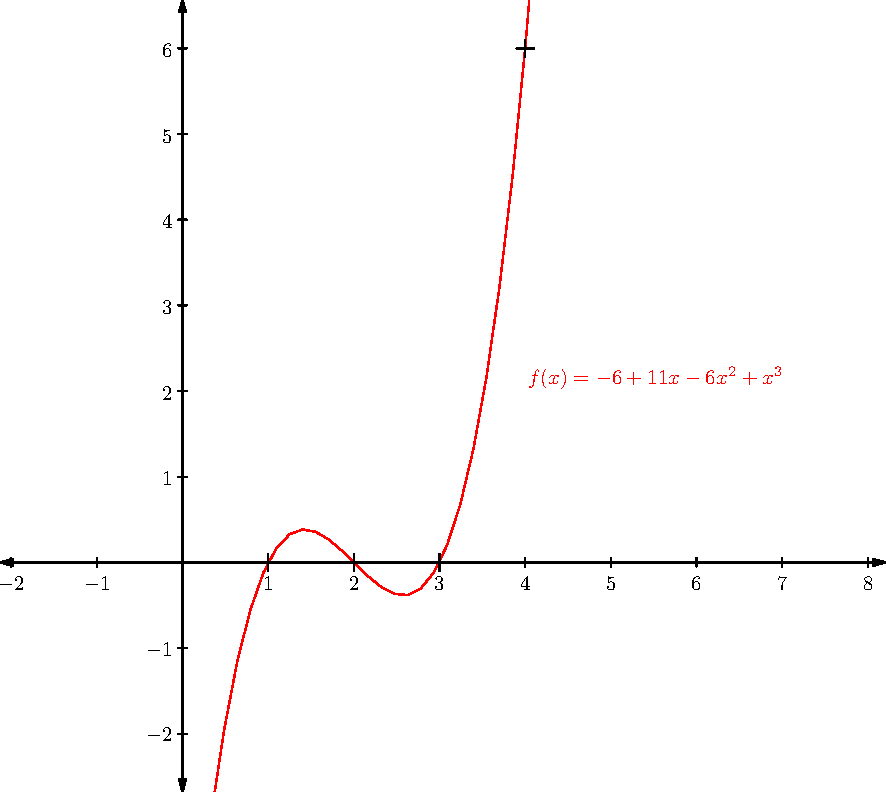
\includegraphics[scale=0.7]{graphiques/pdf_output/inter_test1.pdf}
	\caption{Interpolation de Newton et Neuville -- (Tableau \ref{inter_td3_ex3})}
      \end{figure}
      \newpage
      \begin{table}[h]
	\centering
	\begin{tabular}{| c | c | c | c | c | c | c | c | c | c | c | c |}
	  \hline 
	  $x_{i}$ & $752$ & $855$ & $871$ & $734$ & $610$ & $582$ & $921$ & $492$ & $569$ & $462$ & $907 $ \\ 
	  \hline 
	  $y_{i}$ & $85$ & $83$ & $162$ & $79$ & $81$ & $83$ & $281$ & $81$ & $81$ & $80$ & $243 $ \\ 
	  \hline 
	\end{tabular}
	\caption{Série1 dépense}
	\label{exo_tp3_3}
      \end{table}
      Méthode de Newton : $P(x)= 524166663.148073-8065079.743259 \cdot x + 55479.774423 \cdot x^{2} - 224.689243 \cdot x^{3}  + 0.593281 \cdot x^{4} - 0.001067 \cdot x^{5}  + 0.000001 \cdot x^{6} - 0.000000 \cdot x^{7}  + 0.000000 \cdot x^{8} - 0.000000 \cdot x^{9}  + 0.000000 \cdot x^{10} $
      
      Méthode de Neuville : $P(x)= 524166663.148078-8065079.743259 \cdot x + 55479.774423 \cdot x^{2} - 224.689243 \cdot x^{3}  + 0.593281 \cdot x^{4} - 0.001067 \cdot x^{5}  + 0.000001 \cdot x^{6} - 0.000000 \cdot x^{7}  + 0.000000 \cdot x^{8} - 0.000000 \cdot x^{9}  + 0.000000 \cdot x^{10} $
      
      Pourcentage d'erreur : $0.000046$
      \begin{figure}[h]
	\centering
	%\includegraphics[scale=0.7]{}
	\caption{Interpolation de Newton et Neuville -- (Tableau \ref{exo_tp3_3})}
      \end{figure}
      \renewcommand{\arraystretch}{2}
      \renewcommand{\arraystretch}{1}
    \newpage
    \section{Comparaison}
  \chapter{Approximation}
    \section{Régression linéaire}
      \subsection{Programme}
	\lstinputlisting[style=customc]{reglin.c}
    \newpage
    \section{Résultats de tests}
      \begin{table}[h]
	\centering
	\begin{tabular}{| c | c | c | c | c | c |}
	\hline 
	$x_{i}$ & $0.5$ & $1$ & $1.5$ & $2$ & $2.5$ \\ 
	\hline 
	$y_{i}$ & $0.49$ & $1.6$ & $3.36$ & $6.44$ & $10.16$ \\ 
	\hline 
	\end{tabular}
	\caption{Série 1}
	\label{approx_td3_ex6}
      \end{table}
      \begin{figure}[h]
	\centering
	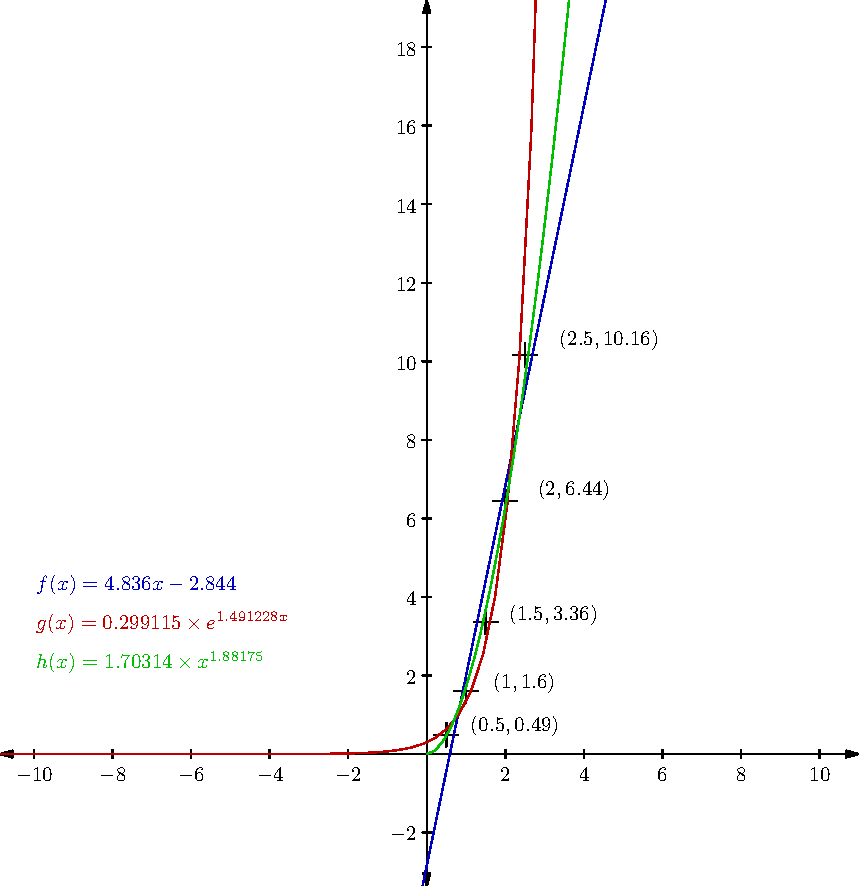
\includegraphics{graphiques/pdf_output/reglin.pdf}
	\caption{Régression linéaire -- (Tableau \ref{approx_td3_ex6})}
      \end{figure}
  \chapter{Conclusion}

\end{document}